\chapter{Modifier les styles bibliographiques (2)}\label{style2}

\renewbibmacro{cite:ibid}{\usebibmacro{cite:full}} % On modifie, pour ne pas avoir des ibidem à tout bout de champs

\begin{intro}
    Nous avons vu que BibLaTeX propose un certain nombre de commandes pour personnaliser rapidement les styles bibliographiques. Toutefois  ces commandes ne suffisent pas pour des personnalisation avancées. 
    La possibilité de choisir l'ordre d'affichage des champs, par exemple, nécessite ainsi d'aller plus loin dans la compréhension des styles bibliographiques de \package{biblatex}.
\end{intro}



\section[Que se passe-t-il lorsqu'on utilise \oldcs{\meta{prefix}cite}]{Que se passe-t-il lorsqu'on utilise une commande \cs{\meta{prefix}cite} ?}

Pour comprendre comment personnaliser l'affichage bibliographique, il est nécessaire de connaître sommairement ce qui se passe lorsqu'on utilise une commande de citation. 


Lorsqu'on appelle une commande de citation, du type \cs{\meta{prefix}cite}, celle-ci va appeler :
    \begin{itemize}
        \item des macros bibliographiques, chargées d'afficher l'argument \arg{prenote} ou \arg{postnote}, ou encore de gérer les citations répétées. Les macros bibliographiques sont des types particuliers de commandes, propres au package \package{biblatex};\label{macrobiblio} 
        \item un driver\footnote{Bien que le terme \enquote{driver} ne soit pas français, nous l'utilisons car on le trouve dans les commandes internes de BibLaTeX} bibliographique. Un driver correspond à un type d'entrée (\type{article}, \type{book}, etc.), et se charge d'afficher les champs de l'entrée dans le bon ordre. Pour cela, il appelle :
        \begin{itemize}
            \item des commandes de séparation d'unités bibliographiques\renvoi{unitebiblio}
, que nous avons vues plus haut;
            \item des macros bibliographiques. Ces macros bibliographiques appellent elles-mêmes :
            \begin{itemize}
                \item des commandes d'impression de champs bibliographiques;
                \item éventuellement d'autres macros bibliographiques;
                \item des chaînes de langues.
            \end{itemize}
        \end{itemize}
        
    \end{itemize}

Ceci peut se résumer par le schéma~\ref{schemastylesbiblios} (p.~\pageref{schemastylesbiblios}). 

\begin{figure}[!]
\begin{center}
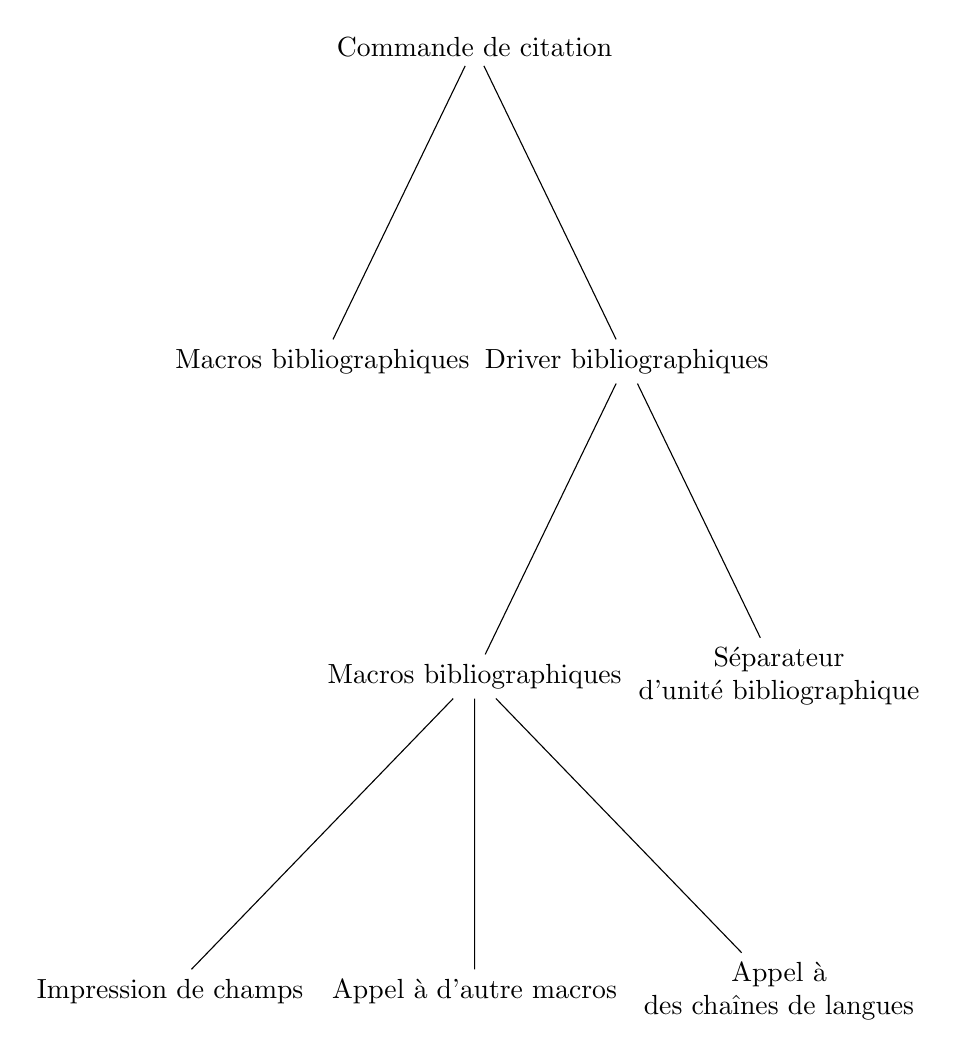
\begin{tikzpicture}[level 1/.style={sibling distance=11em,level distance=4cm},level 2/.style={sibling distance=11em,level distance=4cm},
	every node/.style={align=center}]
	\node {Commande de citation} 
		child { node {Macros bibliographiques}}
		child { node {Driver bibliographiques}
			child { node {Macros bibliographiques}
			 	child {
					node{Impression de champs}
					}
			 	child {
					node{Appel à d'autre macros}
					}
				child {
					node{Appel à \\des chaînes de langues}
					}
				}
			child { node {Séparateur\\ d'unité bibliographique}}
			}	
	;		
\end{tikzpicture}
\end{center}
\caption{Le fonctionnement des styles bibliographiques}\label{schemastylesbiblios}
\end{figure}



\section[Redéfinir une macro bibliographique]{Redéfinir une macro bibliographique : exemple des champs auteur et éditeur}


L'ensemble de ces éléments sont entièrement redéfinissables. Nous allons prendre un exemple concret de problématique existante.

Prenons l'entrée suivante :

\inputminted{exemples/biblio/fichier/saxer.bib}

Elle s'affiche ainsi, avec l'éditeur commercial après l'adresse :

\bibverbose
\begin{quotation}
\cite{Saxer1980}
\end{quotation}


On pourrait souhaiter avoir l'éditeur avant l'adresse, comme ceci : 

\renewbibmacro*{publisher+location+date}{%
  \printlist{publisher}%
    \setunit*{\addcomma\space}%
  \printlist{location}%
  \setunit*{\addcomma\space}%
  \usebibmacro{date}%
  \newunit}

\begin{quotation}
\cite{Saxer1980}
\end{quotation}
\bibverbosetrad


La première chose à faire va donc être de repérer quelle macro bibliographique modifier. Pour cela, il faut trouver les fichiers\renvoi{trouverfichier} de définition des styles bibliographiques. Il en existe plusieurs :

\begin{itemize}
\item un fichier \ext{def} qui définit les styles invariants, quel que soit le style de bibliographie ou de citation choisi;
\item des fichiers \ext{cbx} qui définissent les styles utilisés lors de l'utilisation des commandes \cs{\meta{prefix}cite};
\item des fichiers \ext{bbx} qui définissent les styles utilisés lors de l'appel à la commande \cs{printbibliography}.
\end{itemize}

Certains fichiers s'appellent mutuellement : par exemple les fichiers \ext{bbx} contiennent les drivers bibliographiques. Ils sont donc appelés par les fichiers \ext{cbx}. Ces appels mutuels entre fichiers permettent de garantir une uniformité entre les styles bibliographiques lors de l'utilisation de \cs{\meta{prefix}cite} et lors de l'utilisation de \cs{printbibliography}.

Nous supposons que  vous utilisez les styles de la famille \forme{verbose}. En ouvrant les fichiers standards\renvoi{trouverfichier}, vous pouvez aisément remonter au fichier \fichier{standard.bbx}, qui contient les drivers bibliographiques de cette famille.
Vous pouvez  repérer dedans les lignes suivantes\footnote{L.~58 au 9 octobre 2011.} :

\inputminted{exemples/biblio/styles2/driverbook.tex}

Il s'agit d'un driver bibliographique expliquant comment afficher les entrées de type \type{book}. Il fait appel à des macros bibliographiques \emph{via} les commandes \csp{usebibmacro}. Ces macros sont communes à plusieurs drivers, ce qui permet d'avoir une certaine uniformité de style, afin par exemple que les noms d'auteurs s'affichent systématiquement de la même façon.

Dans le lot des macros appelées, il en existe un qui nous intéresse en particulier, l'appel à la macro \bibmacro{publisher+location+date} via :
 
\begin{latexcode*}{firstnumber=27}
\usebibmacro{publisher+location+date}
\end{latexcode*}

En fouillant un peu le même fichier, on repère l'endroit où la macro est définie :

\inputminted{exemples/biblio/styles2/publisher+location+date.tex}

Nous allons commenter succinctement ces lignes, avant d'expliquer comment faire pour inverser l'ordre des deux champs. 

\begin{description}
\item[Ligne 1] La commande \csp{newbibmacro*} indique que l'on déclare une nouvelle macro bibliographique, ici \bibmacro{publisher+location+date}. Pour indiquer qu'on redéfinit une macro déjà existante, il faut utiliser dans le préambule\footnote{Où ailleurs dans le fichier \ext{tex} mais en tout cas pas dans les fichiers standards.} la commande \csp{renewbibmacro*}. La définition de la macro se trouve dans les accolades qui suivent.
\item[Ligne 2] La commande \csp{printlist} indique que l'on affiche un champ qui pourrait se présenter sous forme de liste, c'est à dire où le mot clef \forme{and} a un sens. Ici il s'agit du champ \champ{location}.
\item[Ligne 3] La commande \csp{iflistundef} teste un champ qui pourrait être une liste, ici le champ \champ{publisher}. Si ce champ est vide, il exécute le contenu de la première accolade (ligne 4), sinon celui de la seconde (ligne 5).
\item[Ligne 4] Si donc le champ \champ{publisher} est vide, on crée une nouvelle unité bibliographique\renvoi{unitebiblio}, via  \csp{setunit*},\label{unitepersonalisee} séparée de la précédente par une virgule à laquelle s'ajoute une espace (\csp{addcomma}\csp{space}\renvoin{commandeponctuation}).
\item[Ligne 5] Si le champ \champ{publisher} n'est pas vide, alors on crée une nouvelle unité bibliographique, séparée de la suivante par un deux-points suivi d'une espace (\csp{addcolon}\csp{space}).
\item[Ligne 6] On imprime le champ \champ{publisher}.
\item[Ligne 7] On crée une nouvelle unité bibliographique, séparée de la précédente par une virgule suivie d'une espace. À noter que le champ \champ{publisher} étant vide, on n'a qu'une seule virgule : nous renvoyons à nos explication antérieure sur les commandes de ponctuation\renvoi{commandeponctuation}.
\item[Ligne 8] On appelle une macro qui se charge de l'affichage de la date.
\item[Ligne 9] On crée une nouvelle unité bibliographique. Le signe séparateur est défini par la commande \cs{newunitpunct}\renvoi{newunitpunct}, vue plus haut.
\end{description}

Pour inverser l'ordre de nos champs, il suffit donc de redéfinir la macro en inversant l'ordre d'impression des champs. Au passage, on ne veut plus des deux points comme séparateurs, ce qui nous permet de supprimer un test conditionnel.


\begin{latexcode}
\renewbibmacro*{publisher+location+date}{%
  \printlist{publisher}%
    \setunit*{\addcomma\space}%
  \printlist{location}%
  \setunit*{\addcomma\space}%
  \usebibmacro{date}%
  \newunit}
\end{latexcode}


\newbibmacro*{publisher+location+date}{%
  \printlist{location}%
  \iflistundef{publisher}
    {\setunit*{\addcomma\space}}
    {\setunit*{\addcolon\space}}%
  \printlist{publisher}%
  \setunit*{\addcomma\space}%
  \usebibmacro{date}%
  \newunit}
    % Remettre les champs dans le bon ordre.



Prêtez bien attention aux \% de fin de lignes : les oublier signifie risquer d'avoir des espaces indésirables dans ses références bibliographiques.


\begin{plusloins}

Il  existe d'autres commandes que \cs{printlist} pour afficher des champs : \csp{printname} pour imprimer un champ contenant des noms de personne, et \csp{printfield} pour imprimer un champ ne nécessitant pas de mise en forme particulière.

Pour mieux comprendre quand utiliser l'une ou l'autre de ces commandes, le mieux est de regarder les fichiers standards.

\end{plusloins}
\begin{plusloins}
Si vous utilisez le champ \champ{address} à la place du champ \champ{location}, sachez que le premier est considéré comme un alias du second : autrement dit, utiliser \champ{address} revient à utiliser \champ{location}.

On peut déclarer des nouveaux alias de champ via la commande :

 \csp{DeclareFieldAlias}\marg{alias}\marg{original}.
\end{plusloins}

\section{Autres exemples : des véritables \emph{op. cit.}}

Un des éléments gênants des styles bibliographiques standards de la famille verbose est leur manière de gérer les abréviations universitaires de type \emph{op. cit.} En effet, les styles indiquent les \emph{op. cit.} après avoir affiché l'auteur et le titre. Par exemple :

\begin{quotation}
\bibverbose	
\cite{Urner1952}

\cite{Saxer1980}
\bibverbosetrad

\cite{Urner1952}

\cite{Saxer1980}
\end{quotation}

Si nous n'avons qu'une seule entrée dont Victor Saxer est l'auteur, cela est assez inutile. On pourrait avoir une version abrégée sous la forme :

\bibverbose

\begin{quotation}
\cite{Urner1952}

\cite{Saxer1980}

% Changeons %
\bibverbosetrad
\renewbibmacro*{cite:title}{%
  \printtext[bibhyperlink]{%
   \ifsingletitle{}{\printfield[citetitle]{labeltitle}}%
    \setunit{\nametitledelim}%
    \bibstring[\mkibid]{opcit}}}
% Changeons


\cite{Urner1952}

\cite{Saxer1980}
\end{quotation}

% Rétablissons
\bibverbosetrad
% Rétablissons

Nous allons pour cela modifier les styles de \emph{biblatex}, en utilisant la commande :
\csp{ifsingletitle}\marg{sioui}\marg{sinon}. 

Cette commande vérifie si une entrée est la seule attribuée à son auteur, et renvoie \arg{sioui} si c'est le cas, \arg{sinon} dans le cas contraire. 

Pour la faire fonctionner, il faut passer l'option \option{singletitle=true} au chargement de \package{biblatex}.

\begin{latexcode}
\usepackage[singletitle=true,...]{biblatex}
\end{latexcode}

Une fois ceci fait, il est nécessaire de savoir où appliquer cette commande. Commençons par fouiller le fichier \ext{cbx}, puisqu'il s'agit d'un style pour une commande \cs{\meta{prefix}cite}. Recherchons l'expression \forme{opcit} qui correspond à la chaîne de langue\renvoi{opcit} qui renvoie \forme{op. cit.}.

On la trouve rapidement dans une macro qui s'appelle  \bibmacro{cite:title}.

\begin{english}%en attendant que ce bug soit résolu
\inputminted{exemples/biblio/styles2/citetitle.tex}
\end{english}
Procédons à l'analyse :

\begin{description}
\item[Ligne 1] Le nom de la macro est \bibmacro{cite:title}.
\item[Ligne 2] La commande \csp{printtext} sert à deux chose : à mettre directement un texte en s'assurant que \emph{biblatex} gère la ponctuation ou bien à assembler plusieurs champs dans un seul bloc typographique. Ici, nous avons affaire au second usage : \contenuarg{bibhyperlink} signifie que \package{biblatex} va s'occuper de mettre un lien hypertexte à l'intérieur du document PDF.
\item[Ligne 3] La commande \cs{printfield} imprime un champ. Ici le pseudo-champ \champ{labeltitle} : celui-ci renvoie la valeur du champ \champ{shortitle} s'il est défini, sinon celle de \champ{title}\renvoi{shortfields}. Il l'affiche selon le format \contenuarg{citetitle}\footcite[On pourrait si on voulait définir une autre manière d'afficher ce champ grâce à la commande \cs{DeclareFieldFormat}. Voir][]{biblatex_formating}.
\item[Ligne 4] Nouvelle unité bibliographique, dont le séparateur est défini par la commande \csp{nametitledelim}.
\item[Ligne 5] La commande \csp{bibstring} sert à appeler une chaîne de langue, ici \verb|opcit|. Le premier argument, dont la valeur est ici \contenuarg{\cs{mkibid}}, indique que la chaîne de langue est passée à  \csp{mkibid} avant d'être affichée. Cette commande qu'on peut redéfinir se charge de la mise en forme : nous avons parlé plus haut de la manière de s'en servir pour avoir les abréviations latines\renvoi{mkibid} en italiques.
\end{description}

La ligne qui nous intéresse est donc la ligne 3, puisque nous voulons conditionner l'affichage du champ titre : s'il n'y a qu'une seule œuvre pour l'auteur courant, on peut ne pas l'afficher. Il suffit de redéclarer la macro, en insérant le test conditionnel :

\begin{english}%en attendant que ce bug soit résolu
\inputminted{exemples/biblio/styles2/singletitle.tex}
\end{english}

\begin{plusloins}
Les éditeurs et gérants de revues peuvent très bien définir leurs propres fichiers \ext{cbx} et \ext{bbx} pour obtenir un ensemble cohérent de styles. Ces fichiers, qui contiennent drivers et macros bibliographiques, doivent commencer par certaines commandes : nous renvoyons à la documentation de \emph{biblatex}\footcite{biblatex_fichiers}.
\end{plusloins}

% On rétablis la gestion des ibidems

\renewbibmacro*{cite:ibid}{%
  \printtext{%
    \bibhyperlink{cite\csuse{cbx@lastcite@\thefield{entrykey}}}{%
      \bibstring[\mkibid]{ibidem}}}%
  \ifloccit
    {\global\toggletrue{cbx:loccit}}
    {}}


